%!TEX root = ../report.tex
One of the goals of the USAR challenge was to create a useable map of the environment. 

The problem an agent faces when it needs to find it's way in an unknown environment is called SLAM, for Simulatenous Localization and Mapping. The agent has no map of the environment, and also no way of knowing it's exact location. It needs to infer the map and it's position on the map from the information it gathers from it's sensors throughout time.

Thus, SLAM is a chicken-and-egg problem: without a map it is hard to estimate the agent's position, and without the agent's position it's hard to estimate the map!

In this section we will first examine how the robot keeps track of the state of the world, and then how the SLAM problem can be solved with Extended Kalman Filters. 

\subsection{State}
\label{slam:state}
The state of the world as it is known to the agent is denoted $x$. The value of this set of variables may change over time, as the agent collects sensor data from the environment. The state at time $t$ is denoted $x_{t}$. 

Many variables may be included in the state variable $x$. For the purpose of this work, we will assume that it contains at least the agent's \em{pose} and a \em{map of the environment}. 

In most SLAM approaches, two types of sensor data is collected: \em{environmental measurement data} and \em{control data}. Environmental measurement data collects information about the environment, while control data collects information about the robot within the environment. Environmental measurement data  is denoted $z$ (at a specific point in time $z_{t}$). Examples of environmental sensors available to an agent are laser scanners, sonars and video cameras. Control data and GPS signals. Control data sensors collect information intrinsic to the agent: it's velocity and position. Examples of control sensors are odometry sensors, inertia sensors and global positioning systems.

For the purpose of this paper we are mainly interested in the online SLAM problem, in contrast to the full SLAM problem. Online (or incremental) SLAM seeks to estimate the current pose $x_{t}$ and map $m$:

\begin{equation}
p(x_{t}, m | z_{1:t}, u_{1:t})
\end{equation}

In contrast, the full SLAM problem estimates all poses $x$ and map $m$:

\begin{equation}
p(x_{1:t}, m | z_{1:t}, u_{1:t})
\end{equation}

In practice, the difference is that the full SLAM problem reconsiders the location of all previous poses in estimating the map, while online SLAM treats these as given. The full SLAM problem is computationally much more expensive. Thus for time sensitive applications, such as real time robot control, usually only online SLAM is performed.

The robot's knowledge of it's current state is reflected in the \emph{belief} function. The belief function gives a posterior probability over the state variable. The belief at time $x_t$ is defined as follows:

\begin{equation}
bel(x_t) = p(x_t | z_{1:t}, u_{1:t})
\end{equation}

This belief is usually updated in two steps: once when the control data ($u_t$) is received, and again when new measurement data ($z_t$) is received. The belief of the robot after the control update is called the prediction, denoted $\overline{bel}(x_t)$:

\begin{equation}
\overline{bel}(x_t) = p(x_t | z_{1:t-1}, u_{1:t})
\end{equation}

A general algorithm for calculating beliefs is the \emph{Bayes filter}. It first calculates the prediction $\overline{bel}(x_t)$ by integrating out the possible values of the previous belief $x_{t-1}$ from previous belief $bel(x_{t-1})$ and the expectation of the current state given the previous state and control data $p(x_t|u_t, x_{t-1})$.

\begin{equation}
\overline{bel}(x_t) = \int p(x_t|u_t, x_{t-1})bel(x_{t-1})\mathrm{d}x_{t-1}
\end{equation}

The final step is the measurement update, in which the measurement data $z_t$ is incorporated:

\begin{equation}
bel(x_t) = \eta p(z_t|x_t)\overline{bel}(x_t)
\end{equation}

In the previous formula, $\eta$ is a normalization constant which ensures that $bel(x_t)$ is a proper probability.

\subsection{Gaussian state representation}
It is often convenient to represent the belief of the current state as a multivariate Gaussian. A Gaussian is defined by its mean $\mu$ and covariance $\Sigma$:

\begin{equation}
p(x) = \det(2\pi\Sigma)^{-\frac{1}{2}}\exp{\{-\frac{1}{2}(x - \mu)^T\Sigma^{-1}(x - \mu)\}}
\end{equation}

Gaussian state representations have the advantage of being easily understood and straightforwardly manipulated. This comes with a cost: a Gaussian is unimodal -- there is only one maximum (the mean) possible. This makes Gaussian representations ill suited when there are many different hypothesis distributed across a map. 

In UsarCommander, the state is represented by a 3-dimensional vector: $(x, y, \theta)$ and the corresponding 3-by-3 covariance matrix $\Sigma$. $x$ and $y$ are the respective coordinates of the robot in a global frame, while $\theta$ is the rotation angle of the robot with respect to the $y$ axis.

When the state is represented by a Gaussian, the formulas in the previous section (\ref{slam:state}) can be relatively easily calculated.

\subsection{Scanmatching}
A robot has access to a variety of sensors, as discussed in section~\ref{slam:state}. Many sensors are not very accurate and reliable: odometry sensors yield erroneous values when the robot's wheels spin on a slippery slope, GPS sensors are unreliable indoors, and inertia sensors experience `drift' -- they need to be calibrated every once in a while. Laser range sensors provide an alternative. It measures with high precision the distance to the first object in a certain direction. 

Laser range sensors are often put in a rotating device, which measures the distance to objects on a (often horizontal) plane. A field of view of 180\degree with a 1\degree resolution is common, which yields 181 distance scans. The 181 scans form a point cloud of 181 points. See image \ref{<<from buyu and pfingstorn p41>>}. 

The `scans' that the laser range sensor returns are processed through a scanmatching algorithm. These algorithms compare two scans (or a scan and a map) to see how they relate to each other. The scanmatcher needs to find out the relative change in orientation and position between the two scans.

In the context of this paper, we will focus on the Weighted Scan Matcher, but various other approaches exist. Slamet and Pfingsthorn\cite{ethembabaoglu2007active} provide an excellent overview of various scanmatching algorithms such as Normal Distribution Transform (NDT), Iterative Dual Correspondence (IDC), Metric-based Iterative Closest Point (MbICP) and ICP.

\subsubsection{Weighted Scan Matcher}
The Weighted Scan Matcher (WSM) was introduced by Pfister et al \cite{pfister2002weighted}. In contrast to other scan matchers, the influence of a correspondence between two measurements is weighted with the certainty of how well the two points match. When two point clouds align perfectly, the uncertainty of these matches is zero. This will not generally be the case. Points that have less associated uncertainty will weigh more in the final scan matching result. The Weighted Scan Matcher explicitly models three error sources: the correspondence error, measurement error, and bias. See figure~\ref{fig:pfister2002}. 

\begin{figure}[ht]
  \begin{center}
    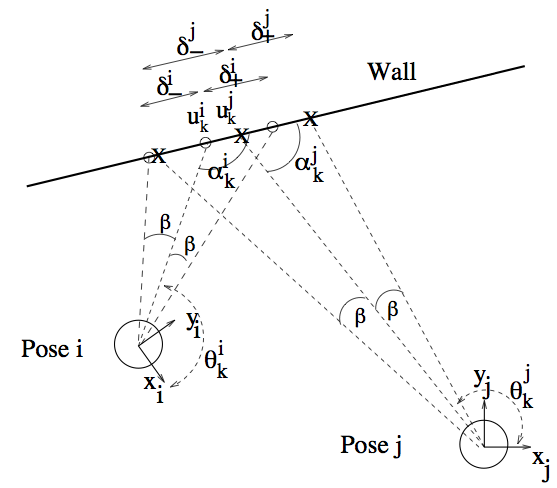
\includegraphics[scale=0.3]{images/slam/pfister2002.png}
  \end{center}
  \caption{Geometry of the scan matching process. Courtesy of \cite{pfister2002weighted}.}
  \label{fig:pfister2002}
\end{figure}

The correspondence error results from the limited resolution available to laser scanners. The resolution in this case is not the resolution in distance measurement, but the angular resolution of the scanner. At a distance of 5 meter and an angular resolution of 1$\degree$, the two measurements lie almost 9 centimeters apart ($500 * \tan(1\degree) \approx 8.7\dots$). When the robot scans again after rotating $0.5\degree$, all measurements will lie in between two previous measurements, and the best match will be off a few centimeters, depending on the distance from the scanner. Even worse: a thin object, such as a iron pole, can be easily missed by the scanning beams as well. All of these errors are examples of the correspondence error.

The measurement error models the error in the measurement process itself. This can because of any external factors which make the measurement erroneous. 

Finally, the bias incorporates the difference between measurement methods. For example, laser scanners and sonar have different performance characteristics. The bias term compensates for this.

In general, the error between two scans $a_i$ and $b_i$ can be expressed as a rotation $R$ and translation $t$:

\begin{equation}
\label{eq:correspondence-error}
\epsilon = a_i - R \cdot b_i - t
\end{equation}

With the assumption that all noise is Gaussian, measurement $a_i$ can be expressed as the addition of the measurement error $\delta r_{a, i}$ and bias error $d_{a, i}$  to the actual distance $r_i$ (similar for $b_i$):

\begin{equation}
\label{eq:measurement}
a_i = r_{a,i} + \delta r_{a, i} + d_{a, i}
\end{equation}

By substituting equation~\ref{eq:measurement} into equation~\ref{eq:correspondence-error}, the full error term is obtained:

\begin{eqnarray}
\epsilon &=& (r_{a,i} + \delta r_{a, i} + d_{a, i}) - R \cdot (r_{b,i} + \delta r_{b, i} + d_{b, i}) - t
			 \nonumber \\
         &=& \underbrace{(r_{a, i} - R \cdot r_{b, i} - t)}_\text{correspondence error} + 
             \underbrace{(\delta r_{a, i} - R \cdot \delta r_{b, i})}_\text{measurement error} + 
             \underbrace{(d_{a, i} - R \cdot d_{b, i})}_\text{bias}
\end{eqnarray}




\subsection{ManifoldSLAM}
Many SLAM algorithms use a bayesian filter to refine the state by incorporate the current knowledge into a new assessment of the current state of the robot. The SLAM algorithm in use by the AJORF team takes the map $m_{t-1}$ and previous position $x_{t-1}$ as given. 


\subsection{2D slam in 3D environment}
Only a slice of the world is returned - so we need to make sure we are horizontal. Otherwise, the scanner returns wrong readings.


UNCERTAINTY MEASURE BY ARNOUD:
To see if the reduced correlation distance also improves the robustness of
the scan matcher the uncertainty measures returned by the algorithms were
analyzed. This uncertainty measure is the full 3-by-3 covariance matrix of the
Gaussian distribution over the displacement estimate and does not lend itself well
for charting in its original form. Therefore we took the on-diagonal elements that
describe the independent uncertainty in x and y direction and combined these
into a Euclidean distance measure. The trace of the covariance matrix acquired
with Q-WSM is in most cases (94%) smaller than the trace of incremental version. The average uncertainty of the Q-WSM algorithm reduced to 36% of the
average uncertainty of the incremental version.


